\begin{refsection}

\chapter{U--Pb geochronology}\label{ch:U-Pb}

\section{Input formats}
\label{sec:UPbFormats}

\texttt{IsoplotR} offers eight different input formats:
\begin{enumerate}
  \item
  $\frac{07}{35}$,  
  $\mbox{err}\!\left[\frac{07}{35}\right]$, 
  $\frac{06}{38}$,  
  $\mbox{err}\!\left[\frac{06}{38}\right]$,  
  $\mbox{r}\!\left[\frac{06}{38},\frac{06}{38}\right]$
  \item $\frac{38}{06}$,  
  $\mbox{err}\!\left[\frac{38}{06}\right]$, 
  $\frac{07}{06}$,  
  $\mbox{err}\!\left[\frac{07}{06}\right]$,  
  $\left(\mbox{r}\!\left[\frac{38}{06},\frac{07}{06}\right]\right)$
  \item
  $\frac{07}{35}$,  
  $\mbox{err}\!\left[\frac{07}{35}\right]$, 
  $\frac{06}{38}$,  
  $\mbox{err}\!\left[\frac{06}{38}\right]$, 
  $\frac{07}{06}$,  
  $\mbox{err}\!\left[\frac{07}{06}\right]$, 
  $\left(\mbox{r}\!\left[\frac{07}{35},\frac{06}{38}\right]\right)$,  
  $\left(\mbox{r}\!\left[\frac{07}{35},\frac{07}{06}\right]\right)$, 
  $\left(\mbox{r}\!\left[\frac{06}{38},\frac{07}{06}\right]\right)$
  \item 
  $\frac{07}{35}$,  
  $\mbox{err}\!\left[\frac{07}{35}\right]$, 
  $\frac{06}{38}$,  
  $\mbox{err}\!\left[\frac{06}{38}\right]$,  
  $\frac{04}{38}$,  
  $\mbox{err}\!\left[\frac{04}{38}\right]$, 
  $\left(\mbox{r}\!\left[\frac{07}{35},\frac{06}{38}\right]\right)$,  
  $\left(\mbox{r}\!\left[\frac{07}{35},\frac{04}{38}\right]\right)$, 
  $\left(\mbox{r}\!\left[\frac{06}{38},\frac{04}{38}\right]\right)$
  \item 
  $\frac{38}{06}$,  
  $\mbox{err}\!\left[\frac{38}{06}\right]$, 
  $\frac{07}{06}$,  
  $\mbox{err}\!\left[\frac{07}{06}\right]$,  
  $\frac{04}{06}$,  
  $\mbox{err}\!\left[\frac{04}{06}\right]$, 
  $\left(\mbox{r}\!\left[\frac{38}{06},\frac{07}{06}\right]\right)$,  
  $\left(\mbox{r}\!\left[\frac{38}{06},\frac{04}{06}\right]\right)$, 
  $\left(\mbox{r}\!\left[\frac{07}{06},\frac{04}{06}\right]\right)$
  \item 
  $\frac{07}{35}$,  
  $\mbox{err}\!\left[\frac{07}{35}\right]$, 
  $\frac{06}{38}$,  
  $\mbox{err}\!\left[\frac{06}{38}\right]$,  
  $\frac{04}{38}$,  
  $\mbox{err}\!\left[\frac{04}{38}\right]$,  
  $\frac{07}{06}$,  
  $\mbox{err}\!\left[\frac{07}{06}\right]$, 
  $\frac{04}{07}$,  
  $\mbox{err}\!\left[\frac{04}{07}\right]$,  
  $\frac{04}{06}$,  
  $\mbox{err}\!\left[\frac{04}{06}\right]$
  \item 
  $\frac{07}{35}$,  
  $\mbox{err}\!\left[\frac{07}{35}\right]$, 
  $\frac{06}{38}$,  
  $\mbox{err}\!\left[\frac{06}{38}\right]$,  
  $\frac{08}{32}$,  
  $\mbox{err}\!\left[\frac{08}{32}\right]$,  
  $\frac{32}{38}$,  
  $\mbox{err}\!\left[\frac{32}{38}\right]$,  \\
  $\left(\mbox{r}\!\left[\frac{07}{35},\frac{06}{38}\right]\right)$,  
  $\left(\mbox{r}\!\left[\frac{07}{35},\frac{08}{32}\right]\right)$, 
  $\left(\mbox{r}\!\left[\frac{07}{35},\frac{32}{38}\right]\right)$,  
  $\left(\mbox{r}\!\left[\frac{06}{38},\frac{08}{32}\right]\right)$,  
  $\left(\mbox{r}\!\left[\frac{06}{38},\frac{32}{38}\right]\right)$, 
  $\left(\mbox{r}\!\left[\frac{08}{32},\frac{32}{38}\right]\right)$
  \item
  $\frac{38}{06}$,  
  $\mbox{err}\!\left[\frac{38}{06}\right]$, 
  $\frac{07}{06}$,  
  $\mbox{err}\!\left[\frac{07}{06}\right]$,  
  $\frac{08}{06}$,  
  $\mbox{err}\!\left[\frac{08}{06}\right]$,  
  $\frac{32}{38}$,  
  $\mbox{err}\!\left[\frac{32}{38}\right]$,  \\
  $\left(\mbox{r}\!\left[\frac{38}{06},\frac{07}{06}\right]\right)$,  
  $\left(\mbox{r}\!\left[\frac{38}{06},\frac{08}{06}\right]\right)$, 
  $\left(\mbox{r}\!\left[\frac{38}{06},\frac{32}{38}\right]\right)$,  
  $\left(\mbox{r}\!\left[\frac{07}{06},\frac{08}{06}\right]\right)$,  
  $\left(\mbox{r}\!\left[\frac{07}{06},\frac{32}{38}\right]\right)$, 
  $\left(\mbox{r}\!\left[\frac{08}{06},\frac{32}{38}\right]\right)$
\end{enumerate}

\noindent where 04, 06, 07, 08, 32, 35 and 38 stand for
\textsuperscript{204}Pb, \textsuperscript{206}Pb,
\textsuperscript{207}Pb, \textsuperscript{208}Pb,
\textsuperscript{232}Th, \textsuperscript{235}U and
\textsuperscript{238}U, respectively. `err[$\ast$]' stands for the
analytical uncertainty of $\ast$, which can be specified as a standard
error or as two times the standard error, either in absolute or
relative units. And `r[$x$,$y$]' stands for the error correlation
between $x$ and $y$.\\

Formats~1--3 are meant for mass spectrometers that are unable to
accurately measure \textsuperscript{204}Pb. This is the case for
single collector ICP-MS instruments that are unable to resolve the
isobaric interference on \textsuperscript{204}Hg, which is often
present in the plasma gas. Formats~4--6 include
\textsuperscript{204}Pb, as measured by SIMS, TIMS or multi-collector
ICP-MS. Finally, formats~7 and 8 include \textsuperscript{208}Pb and
\textsuperscript{232}Th. These nuclides can be used for hybrid
U--Th--Pb dating, as discussed in Section~\ref{sec:U-Th-Pb}.\\

Formats~1, 4 and 7 are `Wetherill style' input formats, in which the
radioactive parent appears in the denominator of the isotopic ratio
data. As explained in Section~\ref{sec:errorcorrelations} and shown in
Figure~\ref{fig:errorcorrelation}, these formats are associated with
strong error correlations
($r\left[\frac{07}{35},\frac{06}{38}\right]$), which must be specified
so as to avoid inaccurate inferences.  Formats~2, 5 and 8 are
`Tera-Wasserburg style' input formats, in which the most abundant
radiogenic daughter (i.e., \textsuperscript{206}Pb) appears in the
denominator of the isotopic ratio data.  As shown in
Figure~\ref{fig:inverrorcorrelation}, this greatly reduces the error
correlations which, consequently, are optional (hence the brackets
around $r\left[\frac{38}{06},\frac{07}{06}\right]$).\\

Finally, formats~3 and 6 provide an alternative input format designed
for users whose low level data processing software does not provide
error correlation data. It uses redundant ratios to infer the
correlation coefficients. Let $X \equiv \frac{07}{35}$, $Y \equiv
\frac{07}{35}$, $Z \equiv \frac{07}{06}$ and $U \equiv \frac{38}{35}$,
let $s[X]$, $s[Y]$ and $s[Z]$ be the standard errors of $X$, $Y$ and
$Z$, and assume that $s[U]=0$ for the sake of simplicity. Then it is
easy to see that $Z = X/(U Y)$, and
\begin{equation}
  \left(\frac{s[Z]}{Z}\right)^2 = \left(\frac{s[X/Y]}{X/Y}\right)^2
  \approx \left(\frac{s[X]}{X}\right)^2 + \left(\frac{s[Y]}{Y}\right)^2 -
  2 \frac{s[X,Y]}{XY}
\end{equation}

\noindent from which the covariance (and, hence, the correlation
coefficient) between $X$ and $Y$ can be inferred as
\begin{equation}
  s[X,Y] \approx \frac{XY}{2}
  \left[
    \left(\frac{s[X]}{X}\right)^2 +
    \left(\frac{s[Y]}{Y}\right)^2 -
    \left(\frac{s[Z]}{Z}\right)^2
    \right]
\end{equation}

It is important to note that this approach makes the crucial
assumption that all three standard errors ($s[X]$, $s[Y]$ and $s[Z]$)
are based on the same number of data points. This means that formats~3
and 6 are not applicable to TIMS data.

\section{Concordia diagrams and ages}
\label{sec:concordia}

\texttt{IsoplotR} implements three types of concordia diagram:

\begin{enumerate}
\item The \textbf{Wetherill} concordia diagram sets out the
  \textsuperscript{206}Pb/\textsuperscript{238}U vs. the
  \textsuperscript{207}Pb/\textsuperscript{235}U ratios. This format
  introduces relatively strong error correlations (see
  Section~\ref{sec:errorcorrelations}). The addition of common Pb
  pulls samples away from concordia along a line whose slope is
  proportional to the common Pb composition. Isotopic compositions
  above the concordia line are `forbidden'. They could, in principle,
  be caused by U-loss. But in practice this mechanism is implausible.
\item The \textbf{Tera-Wasserburg} concordia diagram uses the inverse
  isochron ratios \textsuperscript{207}Pb/\textsuperscript{206}Pb vs.
  and \textsuperscript{238}U/\textsuperscript{206}Pb. This format
  exhibits weaker error correlations. The addition of common Pb
  creates a binary mixing line between radiogenic and common Pb
  compositions (see Section~\ref{sec:discordia}). The area below the
  concordia line is `forbidden' and the only reason why samples may
  plot there is due to random chance and analytical imprecision.
\item The \textbf{U--Th--Pb concordia} diagram sets out the
  conventional isochron ratios of
  \textsuperscript{208}Pb/\textsuperscript{232}Th vs.
  \textsuperscript{206}Pb/\textsuperscript{238}U. Like the Wetherill
  diagram, the U--Th--Pb diagram also exhibits strong error
  correlations.  But in contrast with the Wetherill diagram, the
  addition of common Pb does not necessarily create linear trends on
  the U--Th--Pb diagram. Instead, different aliquots may end up on
  either side of the concordia line depending on their Th/U ratio.
\end{enumerate}

The Wetherill and Tera-Wasserburg concordia plots are available to
datasets from any of \texttt{IsoplotR}'s eight input formats,
irrespective of whether the ratios are stored in a Wetherill or
Tera-Wasserburg format. \texttt{IsoplotR} automatically handles the
data conversions internally. The U--Th--Pb concordia plot is only
available for data formats~7 and 8, because these are the only formats
that account for \textsuperscript{208}Pb and \textsuperscript{232}Th.
The remainder of this Chapter will focus on the Wetherill and
Tera-Wasserburg diagrams, except for Section~\ref{sec:common-Pb},
which will briefly mention the U--Th-Pb diagram again.

\noindent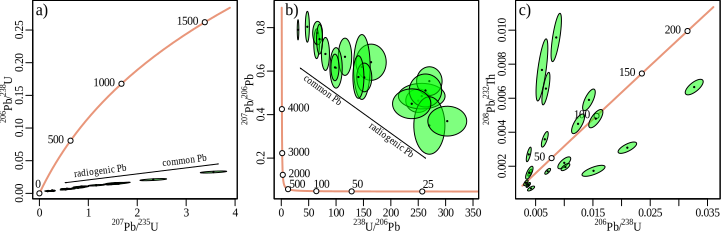
\includegraphics[width=\textwidth]{../figures/3xconcordia.pdf}
\begingroup \captionof{figure}{The allanite dataset of
  \citet{janots2014} shown on a) Wetherill, b) Tera-Wasserburg and c)
  U--Th--Pb concordia diagram.}\endgroup

In the absence of (or after correction for) common Pb or other
complications, multiple aliquots from the same sample may plot on the
concordia line. Such samples are said to be concordant. Their `most
likely' age (in a statistical sense) is known as the \textbf{concordia
  age}. Calculating a concordia age involves two steps
\citep{ludwig1998}:

\begin{enumerate}
  \item Calculate the two-dimensional error-weighted average
    ($\{\bar{x},\bar{y}\}$) of the U--Pb ratios, by maximising the
    likelihood function. In Wetherill space:
    \[
    \mathcal{LL} \propto
    - \sum\limits_{i=1}^{n}
    \left[
      \begin{array}{@{}c@{}}
        \left[\frac{07}{35}\right]_i-\bar{x}\\
        \left[\frac{06}{38}\right]_i-\bar{y}
      \end{array}
      \right]^T
    \left[
      \begin{array}{@{}cc@{}}
        s\!\left[\frac{07}{35}\right]_i^2 &
        s\!\left[\frac{07}{35},\frac{06}{38}\right]_i\\
        s\!\left[\frac{07}{35},\frac{06}{38}\right]_i &
        s\!\left[\frac{06}{38}\right]_i^2
      \end{array}
      \right]^{-1}
    \left[
      \begin{array}{@{}c@{}}
        \left[\frac{07}{35}\right]_i-\bar{x}\\
        \left[\frac{06}{38}\right]_i-\bar{y}
      \end{array}
      \right]    
    \]

    or in Tera-Wasserburg space:
        \[
    \mathcal{LL} \propto
    - \sum\limits_{i=1}^{n}
    \left[
      \begin{array}{@{}c@{}}
        \left[\frac{38}{06}\right]_i-\bar{x}\\
        \left[\frac{07}{06}\right]_i-\bar{y}
      \end{array}
      \right]^T
    \left[
      \begin{array}{@{}cc@{}}
        s\!\left[\frac{38}{06}\right]_i^2 &
        s\!\left[\frac{38}{06},\frac{07}{06}\right]_i\\
        s\!\left[\frac{38}{06},\frac{07}{06}\right]_i &
        s\!\left[\frac{07}{06}\right]_i^2
      \end{array}
      \right]^{-1}
    \left[
      \begin{array}{@{}c@{}}
        \left[\frac{38}{06}\right]_i-\bar{x}\\
        \left[\frac{07}{06}\right]_i-\bar{y}
      \end{array}
      \right]    
    \]

    Using standard maximum likelihood theory, the covariance matrix of
    the weighted mean composition ($\Sigma_{\bar{x},\bar{y}}$) is
    obtained by inverting the matrix of second derivatives of
    $\mathcal{LL}$.
    
  \item Given the concordia composition $\{\bar{x},\bar{y}\}$ obtained
    in the previous step, compute the most likely age ($t_c$) of this
    concordia composition. This is again done using the method of
    maximum likelihood. In Wetherill space:
        \[
    \mathcal{LL} \propto
    - \sum\limits_{i=1}^{n}
    \left[
      \begin{array}{@{}c@{}}
        \bar{x} - (\exp[\lambda_{235}t_c] - 1)\\
        \bar{y} - (\exp[\lambda_{238}t_c] - 1)
      \end{array}
      \right]^T
    \Sigma_{\bar{x},\bar{y}}^{-1}
    \left[
      \begin{array}{@{}c@{}}
        \bar{x} - (\exp[\lambda_{235}t_c] - 1)\\
        \bar{y} - (\exp[\lambda_{238}t_c] - 1)
      \end{array}
      \right]
    \]

    Or in Tera-Wasserburg space:
        \[
    \mathcal{LL} \propto
    - \sum\limits_{i=1}^{n}
    \left[
      \begin{array}{@{}c@{}}
        \bar{x} - \frac{1}{\exp[\lambda_{238}t_c] - 1}\\
        \bar{y} - \left[\frac{35}{38}\right]
        \frac{\exp[\lambda_{235}t_c] - 1}
             {\exp[\lambda_{238}t_c] - 1}
      \end{array}
      \right]^T
    \Sigma_{\bar{x},\bar{y}}^{-1}
    \left[
      \begin{array}{@{}c@{}}
        \bar{x} - \frac{1}{\exp[\lambda_{238}t_c] - 1}\\
        \bar{y} - \left[\frac{35}{38}\right]
        \frac{\exp[\lambda_{235}t_c] - 1}
             {\exp[\lambda_{238}t_c] - 1}
      \end{array}
      \right]^T
    \]

    Again, the uncertainty of $t_c$ is obtained by inverting the
    Fisher information matrix.
    
\end{enumerate}

\noindent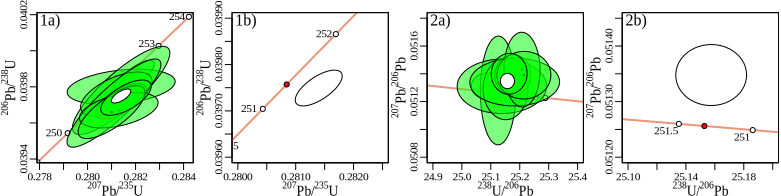
\includegraphics[width=\textwidth]{../figures/concordia_age.pdf}
\begingroup \captionof{figure}{1) Wetherill and 2) Tera-Wasserburg
  concordia diagram with a) the weighted mean composition shown as
  white error ellipse, and b) the maximum concordia age shown as a red
  circle.}\endgroup


\printbibliography[heading=subbibliography]

\end{refsection}
